\documentclass[tikz,border=3mm]{standalone}
\usepackage[T1]{fontenc}
\usepackage{helvet}
\renewcommand{\familydefault}{\sfdefault}
\usepackage{amsmath,amssymb}
\usepackage{tikz}
\usetikzlibrary{shapes.geometric, shapes.misc, positioning,
                arrows.meta, calc}

\begin{document}
%% Flowchart symbols follow ISO 5807:
%%   data (parallelogram): Input/Output
%%   process (rectangle):  assignment
%%   decision (diamond):   condition; each exit from a distinct vertex
%%                         (west/south/east for 3-way; west/east for binary)
%%   connector (filled circle): merge point
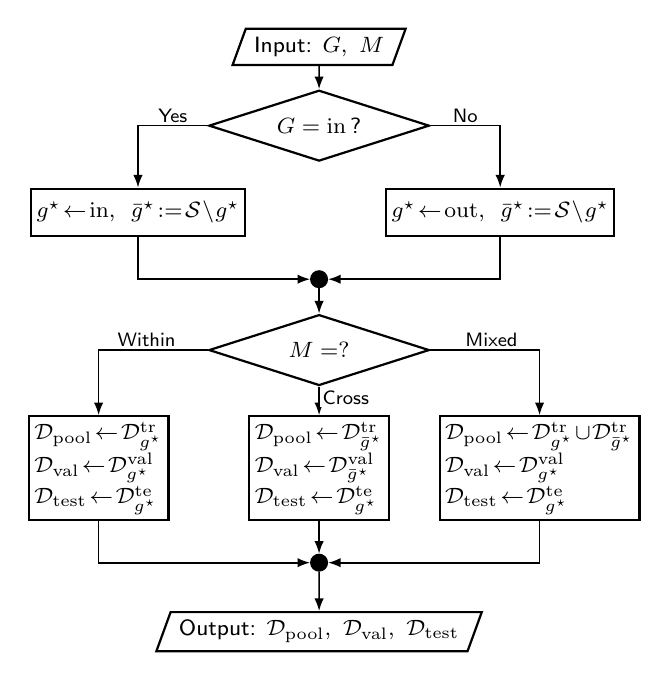
\begin{tikzpicture}[
  every node/.style={font=\sffamily\footnotesize},
  >=Latex,
  data/.style    ={draw, thick, trapezium, trapezium left angle=70,
                   trapezium right angle=110, fill=white, align=center,
                   inner sep=3pt},
  proc/.style    ={draw, thick, rectangle, fill=white, align=center,
                   inner sep=2pt, minimum height=6mm},
  decision/.style={draw, thick, diamond, aspect=2.2, inner sep=0pt,
                   fill=white, align=center},
  merge/.style   ={circle, draw, thick, fill=black, inner sep=0pt,
                   minimum size=2.0mm},
  arr/.style     ={-{Latex[length=1.6mm, width=1.2mm]}, semithick},
  edgelbl/.style ={font=\sffamily\scriptsize, inner sep=1pt, fill=white},
]

%% ---- y layout (all in cm) ----
%%  0.00  Input
%% -1.00  DG  (decision G)
%% -2.10  PGin / PGout   (x = ±2.3)
%% -2.95  mG  (merge after G)
%% -3.85  DM  (decision M)
%% -5.35  PMw / PMc / PMm  (x = -2.8 / 0 / +2.8)
%% -6.55  mM  (merge after M)
%% -7.30  Output

%% ---- Input ----
\node[data] (input) at (0, 0.00) {Input: $G,\ M$};

%% ---- Decision G ----
\node[decision, minimum width=2.8cm, minimum height=0.90cm] (DG) at (0,-1.00)
  {$G = \mathrm{in}$\,?};
\draw[arr] (input) -- (DG);

\node[proc] (PGin)  at (-2.3,-2.10)
  {$g^{\star}\!\leftarrow\!\mathrm{in},\enspace\bar{g}^{\star}\!:=\!\mathcal{S}\!\setminus\!g^{\star}$};
\node[proc] (PGout) at ( 2.3,-2.10)
  {$g^{\star}\!\leftarrow\!\mathrm{out},\enspace\bar{g}^{\star}\!:=\!\mathcal{S}\!\setminus\!g^{\star}$};
\draw[arr] (DG.west) -| node[edgelbl,pos=0.25,above]{Yes} (PGin.north);
\draw[arr] (DG.east) -| node[edgelbl,pos=0.25,above]{No}  (PGout.north);

%% Merge after G
\node[merge] (mG) at (0,-2.95) {};
\draw[arr] (PGin.south)  |- (mG);
\draw[arr] (PGout.south) |- (mG);

%% ---- Decision M (3-way, ISO 5807: west/south/east exits) ----
\node[decision, minimum width=2.8cm, minimum height=0.90cm] (DM) at (0,-3.85)
  {$M = ?$};
\draw[arr] (mG) -- (DM);

%% M=Within (west exit)
\node[proc, align=left] (PMw) at (-2.8,-5.35)
  {$\mathcal{D}_{\mathrm{pool}}\!\leftarrow\!\mathcal{D}^{\mathrm{tr}}_{g^{\star}}$\\[0pt]
   $\mathcal{D}_{\mathrm{val}}\!\leftarrow\!\mathcal{D}^{\mathrm{val}}_{g^{\star}}$\\[0pt]
   $\mathcal{D}_{\mathrm{test}}\!\leftarrow\!\mathcal{D}^{\mathrm{te}}_{g^{\star}}$};
\draw[arr] (DM.west) -| node[edgelbl,pos=0.28,above]{Within} (PMw.north);

%% M=Cross (south exit)
\node[proc, align=left] (PMc) at ( 0.0,-5.35)
  {$\mathcal{D}_{\mathrm{pool}}\!\leftarrow\!\mathcal{D}^{\mathrm{tr}}_{\bar{g}^{\star}}$\\[0pt]
   $\mathcal{D}_{\mathrm{val}}\!\leftarrow\!\mathcal{D}^{\mathrm{val}}_{\bar{g}^{\star}}$\\[0pt]
   $\mathcal{D}_{\mathrm{test}}\!\leftarrow\!\mathcal{D}^{\mathrm{te}}_{g^{\star}}$};
\draw[arr] (DM.south) -- node[edgelbl,pos=0.38,right]{Cross} (PMc.north);

%% M=Mixed (east exit)
\node[proc, align=left] (PMm) at ( 2.8,-5.35)
  {$\mathcal{D}_{\mathrm{pool}}\!\leftarrow\!
    \mathcal{D}^{\mathrm{tr}}_{g^{\star}}\!\cup\!\mathcal{D}^{\mathrm{tr}}_{\bar{g}^{\star}}$\\[0pt]
   $\mathcal{D}_{\mathrm{val}}\!\leftarrow\!\mathcal{D}^{\mathrm{val}}_{g^{\star}}$\\[0pt]
   $\mathcal{D}_{\mathrm{test}}\!\leftarrow\!\mathcal{D}^{\mathrm{te}}_{g^{\star}}$};
\draw[arr] (DM.east) -| node[edgelbl,pos=0.28,above]{Mixed} (PMm.north);

%% Merge after M
\node[merge] (mM) at (0,-6.55) {};
\draw[arr] (PMw.south) |- (mM);
\draw[arr] (PMc.south) -- (mM);
\draw[arr] (PMm.south) |- (mM);

%% ---- Output ----
\node[data, below=5mm of mM] (output)
  {Output: $\mathcal{D}_{\mathrm{pool}},\ \mathcal{D}_{\mathrm{val}},\ \mathcal{D}_{\mathrm{test}}$};
\draw[arr] (mM) -- (output);

\end{tikzpicture}
\end{document}
